\begin{sepframe}{Conclusion}{}
\end{sepframe}

\begin{frame}[fragile,c]
    \frametitle{Composition and inheritance}
    \framesubtitle{Map}

    \makebox[\linewidth]{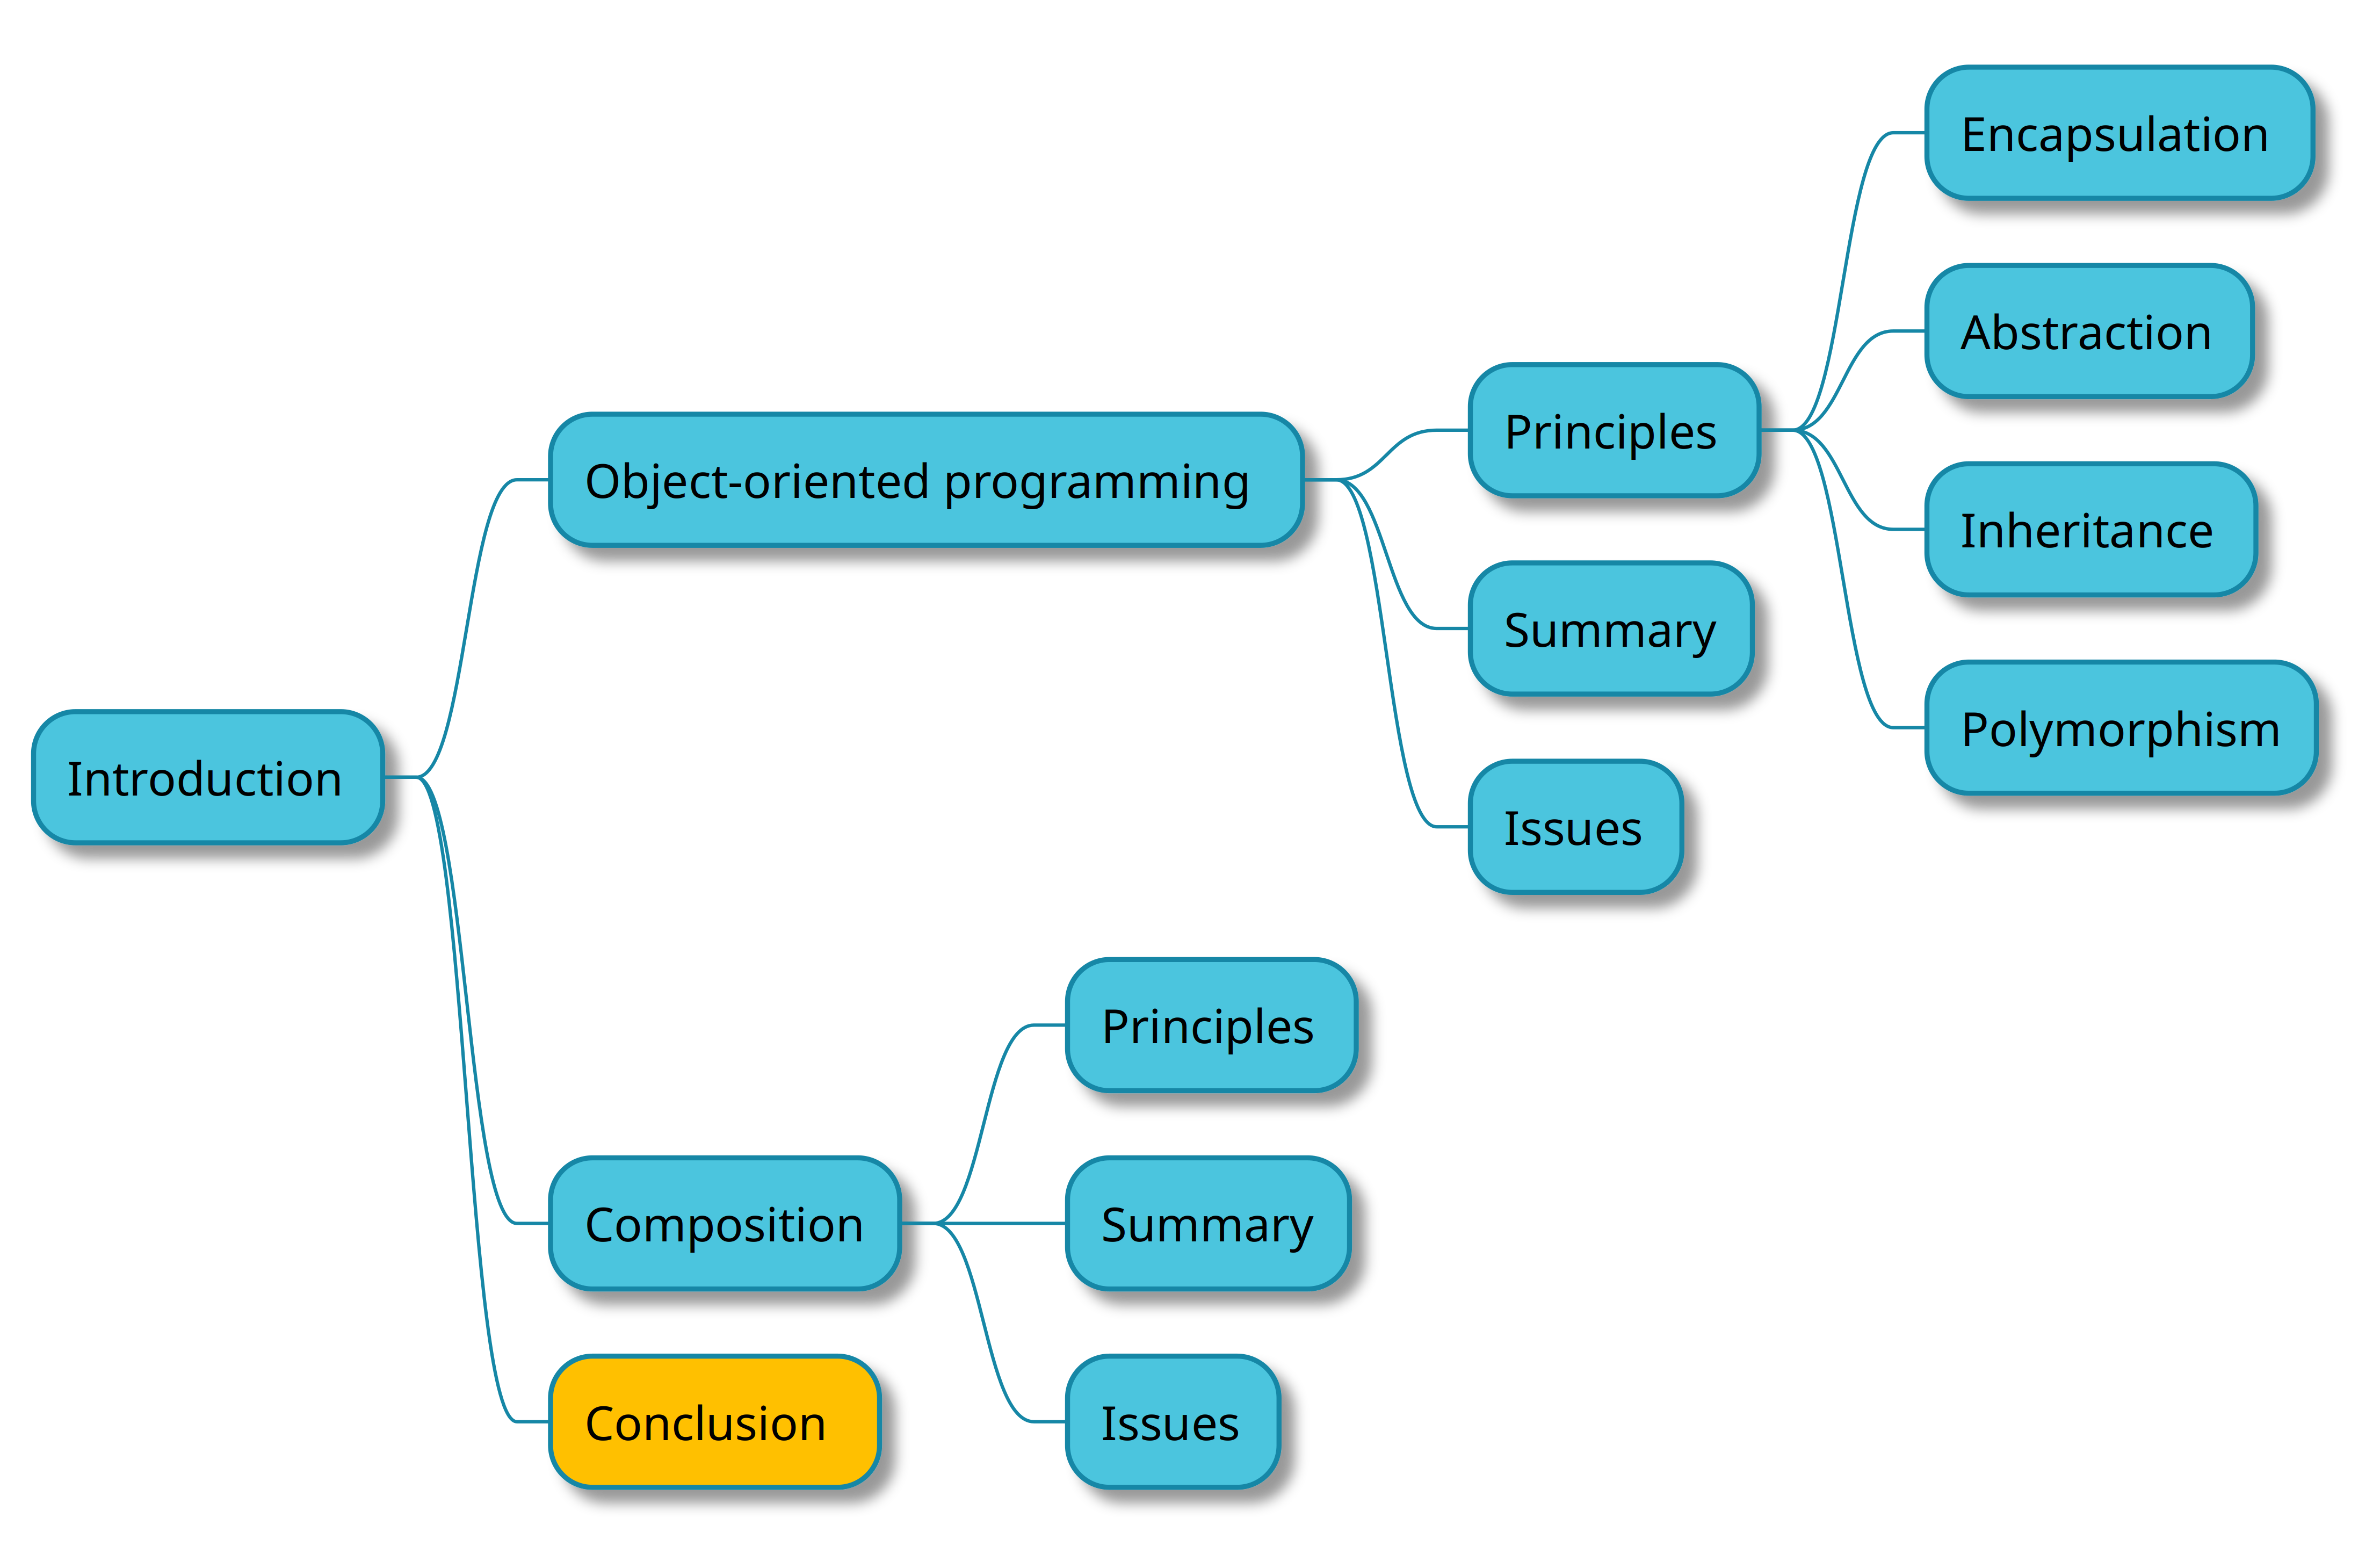
\includegraphics[width=\paperwidth]{src/session--composition-and-inheritance/resources/summary-conclusion.png}}
\end{frame}

\begin{frame}
    \frametitle{Composition and inheritance}
    \framesubtitle{Conclusion / When to use composition?}

    \begin{itemize}[<+->]
        \item Use it everywhere,
        \item As much as you want,
        \item Prefer it to inheritance.
    \end{itemize}
\end{frame}

\begin{frame}
    \frametitle{Composition and inheritance}
    \framesubtitle{Conclusion / Where to use it?}

    \begin{itemize}[<+->]
        \item When customizing part of a framework's component,
        \item When building custom library.
    \end{itemize}
\end{frame}

\begin{frame}[fragile,c]
    \makebox[\linewidth]{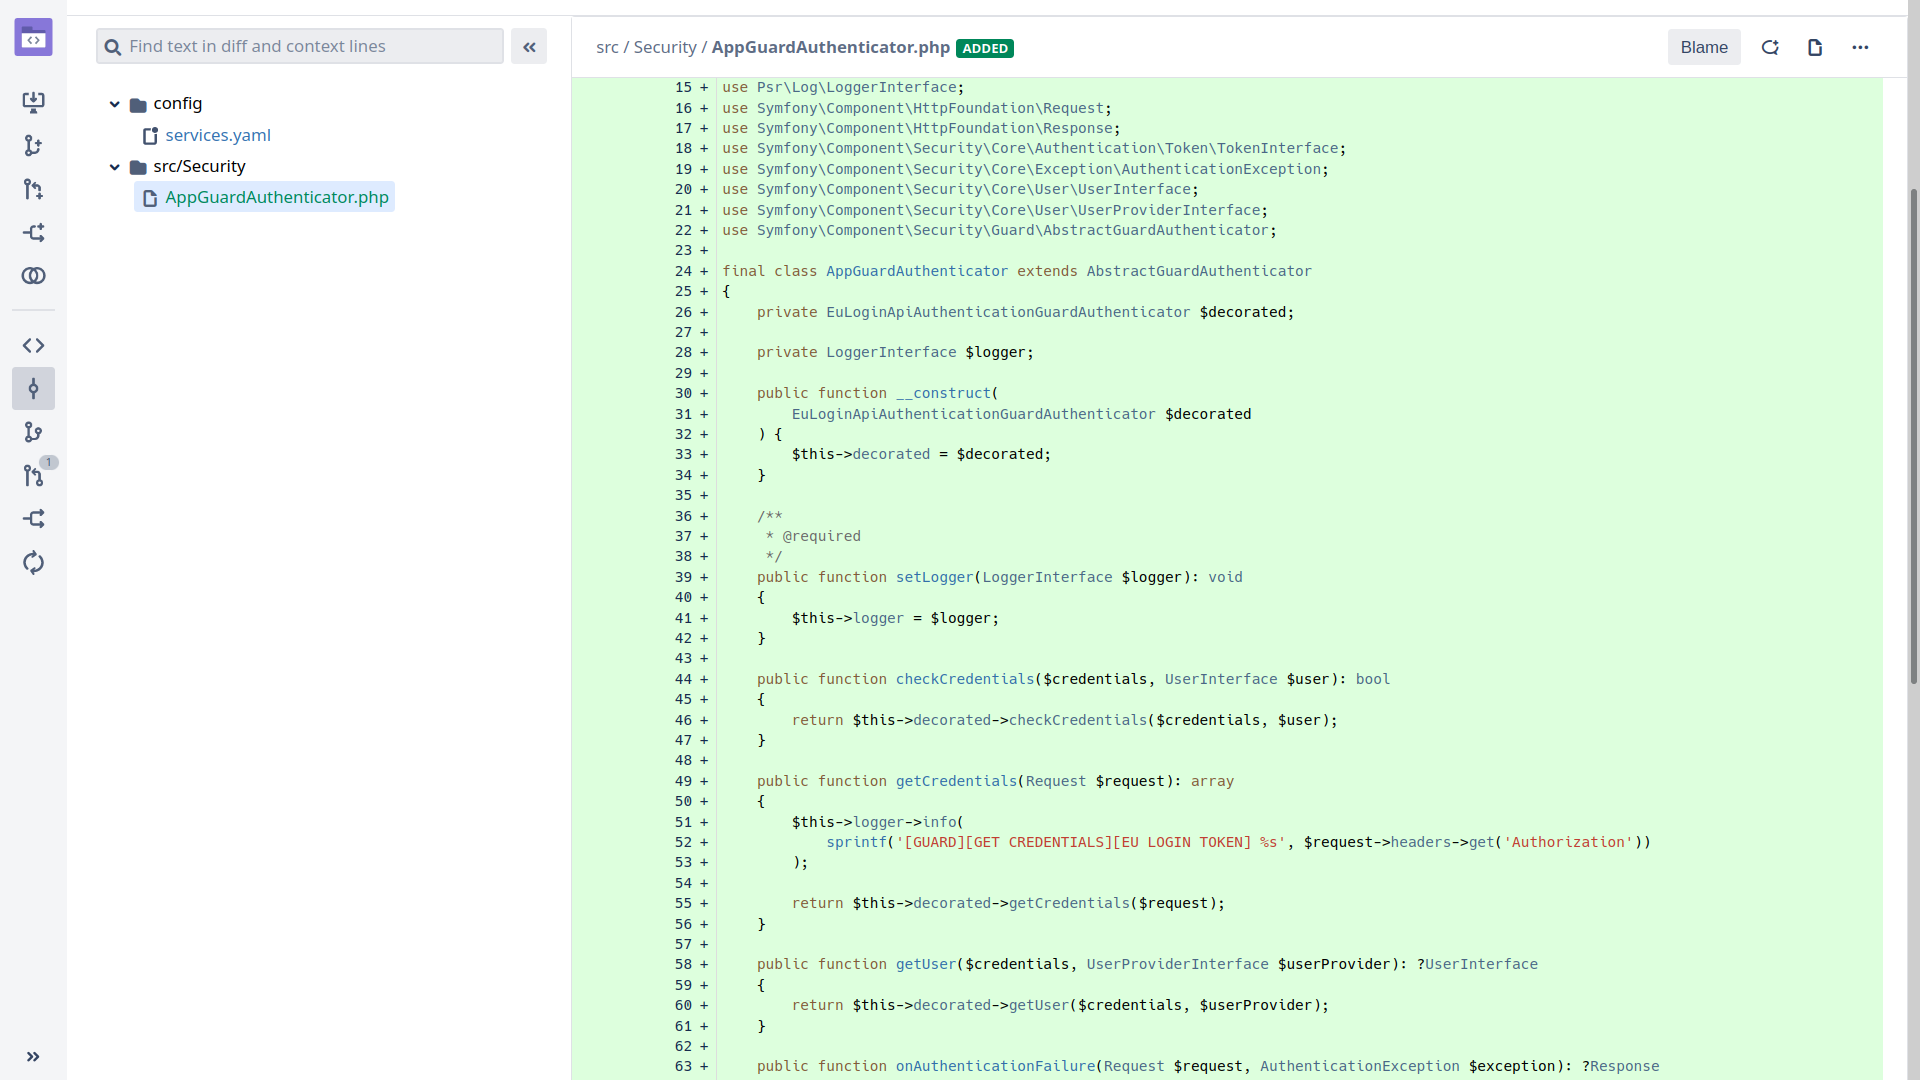
\includegraphics[width=\paperwidth]{src/session--composition-and-inheritance/screenshots/Screenshot_20211108_165811.png}}
\end{frame}

\begin{frame}[fragile,c]
    \begin{lstlisting}
<?php

final class AppGuardAuthenticator extends AbstractGuardAuthenticator
{
    public function __construct(
        private EuLoginApiAuthenticationGuardAuthenticator $decorated,
        private LoggerInterface $logger
    ) {}

    public function getCredentials(Request $request): array
    {
        $this->logger->info(
            sprintf(
                '[GUARD][GET CREDENTIALS][EU LOGIN TOKEN] %s',
                $request->headers->get('Authorization')
            )
        );

        return $this->decorated->getCredentials($request);
    }

    public function checkCredentials($credentials, UserInterface $user): bool
    {
        return $this->decorated->checkCredentials($credentials, $user);
    }
}
    \end{lstlisting}
\end{frame}

\begin{frame}[fragile,c]
    \makebox[\linewidth]{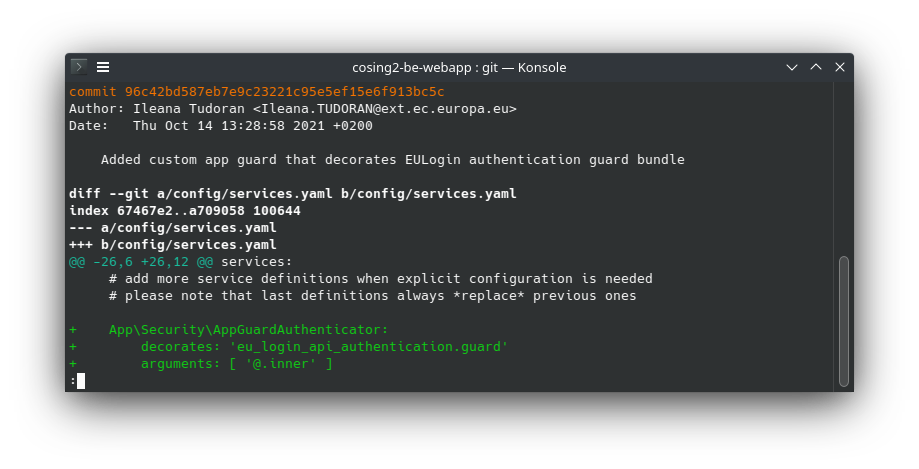
\includegraphics[width=\paperwidth]{src/session--composition-and-inheritance/screenshots/Screenshot_20211108_170213.png}}
\end{frame}

\begin{frame}
    \frametitle{Composition and inheritance}
    \framesubtitle{Conclusion / Advantages of composition over inheritance}

    \begin{itemize}[<+->]
        \item Clearer code,
        \item Ease of testing,
        \item Works well with S.O.L.I.D. principles,
        \item Code instantly fails to run if an updated interface is not fulfilled.
    \end{itemize}
\end{frame}

\begin{frame}
    \frametitle{Composition and inheritance}
    \framesubtitle{Conclusion / Drawbacks of composition over inheritance}

    \begin{itemize}[<+->]
        \item Code is more verbose,
        \item $\cdots$
    \end{itemize}
\end{frame}
